\ifsvnmulti
 \svnkwsave{$RepoFile: siminos/lyapunov/QR.tex $}
 \svnidlong
 {$HeadURL$}
 {$LastChangedDate$}
 {$LastChangedRevision$} {$LastChangedBy$}
 \svnid{$Id$}
\fi

\renewcommand{\ssp}{x}            % state space point

\section{Co-moving frames}
\label{c:comoving}


\subsection{Frenet-Serret frames}
\label{sect:FrenSerr}

\textbf{Challenge:}
Describe here the Frenet-Serret  frames for both group orbits, and
the time-evolution orbit. Might find material from Lautrup\rf{Lau05},
Sect.~10.4 ``Mixed bending and twisting'' and Stone and
Goldbart\rf{StGo09} Exer.~12.10 useful. In particular, read up on the
Fermi-Walker frame used in monomode optical fibers, and the physical
significance of its rotation respective to the Frenet-Serret frame.

\SFIG{LautrupFrenetSerret}
{}{
The Frenet-Serret basis consists of the tangent vector $t$, the normal
$n$ and the binormal $b$. The normal points towards the center of
curvature $C$. As the point $x$ moves along the curve, the basis turns
around b and twists around $t$ to reflect the geometric curvature and
torsion of the oriented curve.
(from Lautrup\rf{Lau05})
}{}

Stone and Goldbart call the frame Serret-Frenet; which usage is right?
Lautrup says ``due to Frenet in 1847 (and independently to Serret in
1851)'', but Serret is more influential mathematician.
                                    \toCB
\emph{[Moved here from ChaosBook, return someday:]}
The eigenvalues and the eigen\-vectors of \stabmat\  ${\Mvar}_\stagn$
evaluated at a stagnation point $\ssp_\stagn$
\index{covariant Lyapunov vector}\index{Lyapunov!covariant vector}
\beq
{\Mvar}_\stagn \, \jEigvec[j](\ssp_\stagn)
   = \eigExp[j]_\stagn \,\jEigvec[j] (\ssp_\stagn)
\,,
\ee{cplxEigExp}
describe the linearized neighborhood of the \eqv\ point, with
$\eigExp[j]_p = \eigRe[j]_p \pm i\eigIm[j]_p$ and $\sign{p}^{(j)}$
independent of any particular coordinate choice.

\exercise{Constant Frenet-Serret  frames.}{\label{e-3-disk-symb}
\index{Frenet-Serret basis}
Prove that if both curvature and torsion are constants
independent of $s$, the curve becomes a perfect helix.
(Lautrup\rf{Lau05} Exer.~10.7)
} % end \exercise{Sensitivity to initial conditions}{

\begin{description}

\item[Predrag 2010-03-25 ]
Gilmore, Ginoux, Jones,
Letellier and Freitas\rf{GGJLF10}, \arXiv{1003.1703}
write: ``
The acceleration vector
\[
\gamma(t) = \frac{d \vel}{dt}
\]
is the time derivative of $\vel(t)$ at the instant $t$. The
chain rule leads to
\[
\gamma_j = \Mvar_{jk}\vel_k
\,.
\]
Gilmore \etal\ go beyond the zero-dimensional invariant sets of \eqva\
and introduce a {\em ``connecting''} curve that passes through  \eqva\ of
the autonomous dynamical system. The {\em ``connecting''} curve  can be
defined in two equivalent ways, (1) dynamically, as a ``vortex core''
curve through the eigenvalue-like equation
\(
\Mvar \, \vel = \Lyap  \, \vel
\,,
\)
and (2) kinematically, as the locus of points in the \statesp\ where the
principal curvature is zero.
''


\item[Predrag 2010-04-05 ]
\emph{From limit cycles to strange attractors}
by
William Ott and Mikko Stenlund,
\HREF{http://arxiv.org/abs/1004.0019}{arXiv:1004.0019}.
They say:
``
We define a quantitative notion of shear for limit cycles of flows. We
prove that strange attractors and SRB measures emerge when systems
exhibiting limit cycles with sufficient shear are subjected to periodic
pulsatile drives. The strange attractors possess a number of
precisely-defined dynamical properties that together imply chaos that is
both sustained in time and physically observable.
''

{\bf Predrag's 2010-04-05 notes:}
They require that $d\ssp/dt = \vel(\ssp)$ is $C^5$, start by looking at
an attractive cycle $p$ of length $L$ parametrized by length parameter
$s$, and let $\gamma : \reals \to \reals^d$ be a function of the
parameter $s$. The define $\Gamma = \{ \gamma(s) : s \in [0,L) \} $ and a
tubular neighborhood $\overline{\pS} =\Gamma \times D$, expressed in the
natural $(s,z )$-coordinates, where $D$ is a closed disk in
$\reals^{d-1}$1 of sufficiently small radius.

What might be of interest is the way they construct local normal basis by
applying the Gram-Schmidt procedure and utilizing the first $n$
derivatives $d^k\gamma(s)/ds^k$ to obtain is a skew-symmetric matrix of
generalized curvatures and identifying the co-moving differential
equation as the classical Frenet-Serret equation from differential
geometry.

\item[ES 2010-01-28]
Here is some stuff from Siminos thesis that might or might not be
relevant in this context:

Predrag dropped this but I am not sure: ``In general, when a \slice\
$\pSRed$ is defined through relations of the form $\overline{x}_i=0$,
$i=1,\ldots,N$ then we call $\pSRed$ a \emph{coordinate \slice}.''

Once a linear \slice\ $\pSRed=\{x_1=c_1,\ldots,x_r=c_N\}$ is defined by
the first $N$ coordinates (relabel coordinates as necessary), we write
the group transformations as
\beq
	\overline{x}= g \cdot x = w(g,x)\,.
	\label{eq:transNorm}
\eeq
Equating the first $N$ components of the function $w$ to the
constants in the definition of the {\slice} $\pSRed_i(x)=c_i$
yields the \emph{slice conditions} for $\pSRed$:
\beq
	\overline{x}_1=w_1(g,x)=c_1,\ldots,\overline{x}_N=w_N(g,x)=c_N\,.
	\label{eq:normalization}
\eeq
The slice conditions \refeq{eq:normalization} can always be
solved\rf{FelsOlver99} for the group parameters in terms of $x$, yielding
the moving frame associated with $\pSRed$: $\LieEl=\LieEl(x)$. For proof
\cf~\refrefs{FelsOlver98,FelsOlver99}. This can be thought of as
generalization of the Frenet-Serret co-moving frame.

\item[ES  2009-05-05]
Fels and Olver claim that ``a moving frame as an equivariant map from a
manifold to a Lie group'' is exactly \emph{their} interpretation of
\mframes\ so I've dropped this: The notion of a {\em moving frame} as a
map from a manifold to a Lie group was introduced by Cartan\rf{CartanMF}.


\item[PC 2012-01-20]                                                \toCB
Cantwell\rf{Cantwell92} {\em Exact solution of a restricted {Euler}
equation for the velocity gradient tensor} might be of interest for
writing up transport in \statesp. It is all about the
Navier-Stokes, 3-dimensional the velocity gradient tensor
\(
{\Mvar}_{ij} ={\pde \vel_i \over \pde \ssp_j  }
\,.\)
For dynamical flows in \statesp\ we call this \velgradmat\ ${\Mvar}$
defined in \refeq{DerMatrix} the {\stabmat}. He writes equations for its
transport, but incompressibility and 3 dimensions seem to be crucial for
everything written there.

Also Chertkov, Pumir and Shraiman\rf{ChePuShr99} might be of interest,
get it \HREF{http://cnls.lanl.gov/~chertkov/Papers/99CPS.pdf}{here}. They
considering the Lagrangian dynamics of 4 points (the \emph{tetrad}). The
closure of the equations of motion is achieved by postulating an
anisotropic, \ie, tetrad shape dependent, relation of the local pressure
and the velocity gradient defined on the tetrad. The non-local
contribution to the pressure and the incoherent small scale fluctuations
are modeled as Gaussian white ``noise''. The resulting stochastic model
for the coarse-grained velocity gradient is analyzed approximately.
Again, incompressibility and 3 dimensions seem to be crucial.

\end{description}

\newpage
\section{Nambu Hamiltonians}
\label{sect:Nambu}

\begin{description}

\item[Predrag 2011-09-17 ]
Nambu Hamiltonians\rf{Nambu73,Takh93} are about 3-dimensional
incompressible flows (such as given by the \eqv\ and \po\ solutions of
\pCf) and belong to Elton blog, but as that blog is currently dormant, I
am provisorily entering my notes here. What is clear from Elton's work is
presence of various KAM-like surfaces, even in the absence of symplectic
structure; the 3D Navier-Stokes flow is volume preserving, but has no
Poincar\'e symplectic $\{q_i,p_i\}$ pairs; Nambu formulation maybe
explains what we see.

The formulation has its origins in the Euler equations for the angular
momentum of a rigid body in three dimensions, which was Nambu's only
example. All known systems share possess dynamical or hidden symmetries
resulting in extra integrals of motion beyond those needed for complete
integrability. Apparently  Nambu formulation is powerful for
``superintegrable systems,'' which is definitely not our situation.
But it might nevertheless come in handy in its linearized version, just as
local quadratic approximations to Hamiltonians are useful (\po\ stability,
Maslov phases \etc) even almost no dynamical system is globally integrable.

Nambu\rf{Nambu73} introduced Poisson bracket for generalized Hamilton
mechanics: Let $(x^i,i=1,2,\cdots, n)$ be a set of dynamical variables
which span a $n$-dimensional phase space. The concept of a Nambu-Poisson
structure was introduced by Takhtajan\rf{Takh93} in order to find an
axiomatic formalism for the $n$-bracket operation
\[
\{f_1, . . . , f_n\} =
\mbox{det} \left( \frac{\partial f_{i}}{\partial x_{j} } \right)
\]
proposed by Nambu\rf{Nambu73} as a generalization of the Hamiltonian
mechanics.
Bit more explicitly, a Nambu-Poisson structure is defined as
\beq
\{f_1, f_2,\cdots, f_n\} =\sum_{i_1,i_2,\cdots,i_n}
\epsilon_{i_1,i_2,\cdots,i_n} \frac{\partial f_1}{\partial x_{i_1}}
\frac{\partial f_2}{\partial x_{i_2}}\cdots \frac{\partial f_n}{\partial x_{i_n}},
\ee{nambupb}
where $\epsilon_{i_1,i_2,\cdots,i_n}$ is the $n$-dimensional Levi-Civita
tensor; generalizing the  $\epsilon_{i_1,i_2,i_3}$ of the $SO(3)$
symmetry of Nambu's rigid body angular momentum. The assumption made by
Takhtajan was that the bracket, acting on smooth functions, has to
satisfy the Leibniz rule.

\item[Predrag 2011-09-17 ] In
\emph{Non Hamiltonian chaos from Nambu dynamics of surfaces}
%{Published in Chaos Theory: Modeling, Simulation and Applications,
%\\C.H. Skiadas, I. Dimotikalis and C. Skiadas (Eds),
%\\World Scientific Publishing Co, pp. 110-119.}   }
Minos Axenides\rf{Axen11}, \arXiv{1109.0470},
(see also \refrefs{AxFl09,AxFlNi09,Flor11})
writes: ``

The Nambu 3-bracket, a generalization of Poisson bracket in
Hamiltonian mechanics, is defined as
\beq
\{ f, g, h \} \ = \ \epsilon^{ijk} \partial^{i}f \partial^{j}g \partial^{k}h
\qquad i,j,k=1,2,3 \quad \forall f,g,h \in C^{\infty}( R^{3})
\ee{Nambu3flow}

Any local coordinate transformation
\beq
x^{i} \ \rightarrow \ y^{i} \ = \ y^{i}(x) \qquad i=1,2,3
\eeq
which preserves the volume of phase space
\beq
\mbox{det} \left( \frac{\partial y^{i}}{\partial x^{j} } \right) \ = \ 1
    \qquad \forall \ x=(x^{1},x^{2},x^{3}) \in R^{3}
\eeq
leaves invariant the 3-bracket and is a symmetry of Nambu mechanics.
Except for the linearity and antisymmetry of the bracket with respect to all of
its arguments it also
satisfies an important identity, the so called Fundamental identity\rf{AxFl09,AxFl08}.

Nambu-Hamiltonian mechanics of a dynamical system in $R^{3}$ is defined by
two scalar functions $H_{i}\in C^{\infty}(R^{3}), i=1,2 $, the generalized
Hamiltonians\rf{Nambu73,Takh93}, with the evolution equations
\beq
\dot{x}^{i} \ = \  \{ x^{i} , H_{1} , H_{2} \} \ \ \ \ \ \ \ \  i=1,2,3
\,.
\eeq
For Lorenz and R\"{o}ssler attractor examples,
the associated linear Nambu maps are generated by a pair of linear
and quadratic Hamiltonians (Clebsch-Monge potentials of the flow).
The evolution \refeq{Nambu3flow} has a flow vector field:
\beq
v^{i}(x) \ \ = \ \ \epsilon^{ijk}\partial^{j} H_{1} \partial^{k}H_{2} \ \ \ \
\ \ \ \ \ i,j,k=1,2,3
\eeq
which is volume preserving
\beq
\partial^{i} v ^{i} \ = \ 0
\eeq
They refer to the phase-space volume preserving flows as
"Non-dissipative", and the non-conserving ones as "Dissipative"
($\partial^{i} v^{i}(x) > 0(< 0))$, and present an investigation of the
Lorenz and R\"{o}ssler attractors from the point of view of Dissipative
Nambu-Hamiltonian Dynamics.

[Predrag: to me the discussion appears not persuasive; not sure that the
decomposition into  Non-dissipative"  and "Dissipative", and what is
gained by going through the exercise. For example, Rupak Chatterjee says
``the definition of these generalized Hamiltonians is not unique.'']


From \refref{AxFlNi09}:
``we believe that the proposed framework of quantization for Nambu
mechanics will lead to new insights for the quantization of volume
preserving diffeomorphism group in 3-dimensions.''

\item[Predrag 2011-09-17 ]
For 3D Navier Stokes, the Nambu Lagrangian seems to be written in
\refref{MiPlSt11}, reproduced here as eq.~\refeq{MiPlSt11:Lagr}.
They write the Navier-Stokes equation as (using the repeated index summation convention)
\begin{equation}
\rho (\partial_t v_i + v_j \partial_j v_i) = - \partial_i p + \nu \partial_j^2 v_i,
\end{equation}
with the incompressibility condition $\partial_i v_i = 0$, where $v_i$ is
a component of the velocity field of the flow, $p$ is pressure, and
$\rho$ is the fluid density. In 3D they consider
\begin{equation}
L_3= \int d^3y \rho_0
\left( \frac{m}{2} \dot{x}^2 - V( \rho_0 |{ \partial y}/{\partial x}|) \right)
\,.
\label{MiPlSt11:Lagr}
\end{equation}
The Lagrangian $L_3$ is invariant under volume preserving diffeomorphisms
\begin{equation}
\delta x_a = \frac{\partial x_a}{\partial y_i}\epsilon_{ijk} \frac{\partial \Lambda_1(y)}{\partial y_j}
\frac{\partial \Lambda_2(y)}{\partial y_k}.
\end{equation}
where $\Lambda_1$ and $\Lambda_2$ are the generators of the volume preserving
gauge transformations.
This is equivalent to the following Nambu bracket\rf{Nambu73}:
\begin{equation}
\delta x_a \equiv \{\Lambda_1, \Lambda_2, x_a\},
\end{equation}
where, by definition
\begin{equation}
\{A, B, C\}\equiv \epsilon_{abc} \partial_a A \partial_b B \partial_c C.
\end{equation}
Here $A,B,C$ are three functions of three spatial coordinates $x,y,z$.
This classical bracket seems to be naturally generalized to a triple
algebraic structure\rf{Nambu73} %, triples, vector}
\begin{equation}
[A_i, A_j, A_k] \equiv \epsilon_{abc} A_a A_b A_c
\end{equation}
They consider small motions of the 3d fluid:
\begin{equation}
x_i = y_i + f \epsilon_{ijk} B_{jk},
\end{equation}
where $B_{jk}= - B_{kj}$ and $f$ denotes a small coupling.
The 3D action invariant under the linear part of this transformation is
\begin{equation}
S_B = \frac{1}{2 f^2}  \int d^3y [  \dot{B}_{ij}^2 - (\partial_i B_{jk} +\partial_j B_{ki} +\partial_k B_{ij})^2].
\end{equation}
Note that the explicit linear volume preserving transformations are
\begin{equation}
\delta B_{ij} = \partial_i \Lambda_1 \partial_j \Lambda_2 - \partial_i \Lambda_2
\partial_j \Lambda_1,
\end{equation}
where $B_{ij}$  is dual to a 3-vector in three dimensions,
$
a_i = \frac{1}{2} \epsilon_{ijk} B_{jk}
$.
[Predrag: the rest is Kraichnan, Kolmogorov kind of statistics arguments that
we prefer not to get into.]

\item[Christel 2011-10-05 ] This could be interesting for the symmetry
reduction in a Hamiltonian context of a rather simple model.
Z. Roupas\rf{Roupas11} says in
\emph{Symmetries of phase space flow and chaotic attractors},
 \arXiv{1110.0766}: ``
Following the Nambu mechanics framework we demonstrate that the
non-dissipative part of the Lorenz system can be generated by the
intersection of two quadratic surfaces that form a doublet under the
group $SL(2,R)$. All manifolds are classified into four distinct classes;
parabolic, elliptical, cylindrical and hyperbolic. The Lorenz attractor
is localized by a specific infinite set of one parameter family of these
surfaces. The different classes correspond to different physical systems.
The Lorenz system is identified as a charged rigid body in a uniform
magnetic field with external torque and this system is generalized to
give new strange attractors.
''

Roupas\rf{Roupas11} was renamed \emph{Phase Space Geometry and Chaotic
Attractors in Dissipative Nambu Mechanics} in the published version.

\item[Predrag 2012-02-23 ]
Richard Blender and Valerio Lucarini say  in
\emph{Nambu representation of an extended Lorenz model with viscous heating},
 \arXiv{1202.2210}: ``
We consider the Nambu and Hamiltonian representations of Rayleigh-Benard
convection with a nonlinear thermal heating effect proportional to the
Eckert number (Ec). The model we use is an extension of the classical
Lorenz-63 model with 4 kinematic and 6 thermal degrees of freedom. The
conservative parts of the dynamical equations which include all
nonlinearities satisfy Liouville's theorem and permit a conserved
Hamiltonian H for arbitrary Ec. For Ec=0 two independent conserved
Casimir functions exist, one of these is associated with unavailable
potential energy and is also present in the Lorenz-63 truncation. This
Casimir C is used to construct a Nambu representation of the conserved
part of the dynamical system. The thermal heating effect can be
represented either by a second canonical Hamiltonian or as a gradient
(metric) system using the time derivative of the Casimir. The results
demonstrate the impact of viscous heating in the total energy budget and
in the Lorenz energy cycle for kinetic and available potential energy.
 ''


\end{description}

\newpage
\section{Stability in a co-moving frame}
\label{sect:stabComoving}
% Predrag                           		2011-03-05
% moved to here halcrow/blog/TEX/QR.tex		2008-12-07

{\bf Predrag 2011-03-05}
{These appendices contain material that will eventually be returned back to
    ChaosBook.org. Please keep ChaosBook formatting throughout this chapter.
    Thanks!}

%%%%%%%%%%%%%%%%%%%%%%%%%%%%%%%%%%%%%%%%%%%%%%%%%%%%%%%%%%%%%%%%%%%%%%%%%%
\exercise{Stability in a co-moving frame.}{ \label{exer:stabComoving}
% Predrag                           19feb2008
\index{stability|co-moving frame}
\index{|co-moving frame|stability}
    %
\PC{ChaosBook: add this to Problems/exerAppApplic}
%
The {\em \stabmat}(velocity gradient matrix):
\index{matrix!stability}
\index{stability!matrix}
\index{velocity gradient matrix}
% % http://mathworld.wolfram.com/StabilityMatrix.html
% calls this `stability matrix'.
%   }
\beq
{\Mvar}_{ij}(\ssp) = \frac{\pde \vel_i(\ssp)}{\pde \ssp_j  }
\ee{appl:DerMatrix}
The linearized neighborhood is transported by the
{\jacobianM}
% This Jacobian matrix has inherited the name
% {\em fundamental solution matrix} or simply
% {\em fundamental matrix}
% from the theory of linear ODEs.
\index{fundamental matrix}
\beq
\jMps^t_{ij}(\xInit)
  =  \left. {\pde \ssp_i(t) \over \pde \ssp_j} \right|_{\ssp=\xInit}
\, .
\label{appl:hOdes}
\eeq
$\ExpaEig_k$ denotes
the $k$th
{\em eigen\-value}
(multiplier)
 of the finite time
 {\jacobianM} $\jMps^t$,
\index{stability!eigenvalue}
while $\eigExp[k]$ denotes
the $k$th {\em characteristic exponent}
or
{\em characteristic value},
% sometimes the same thing as the {\em Lyapunov exponent}),
with real part $\eigRe[k]$
% is sometimes the same thing as the {\em Lyapunov exponent}),
and phase $\eigIm[k]$:
\index{characteristic!exponent}
\index{characteristic!value}
% \index{Lyapunov exponent}
\beq
\ExpaEig_k
 =
e^{t \eigExp[k]}
 =
e^{t\eigRe[k] +i t\eigIm[k]}
\,.
\ee{appl:stabExpon}
$\derf{t}{\xInit}$ depends on the initial point $\xInit$
and the elapsed time $t$. For notational brevity we tend to
omit this dependence. Projection operator
\beq
{\PP}_i = \prod_{j\not= i}
   \frac{\jMps-\ExpaEig_j \matId }
        {\ExpaEig_i - \ExpaEig_j} \, ,
\ee{appl:stab:3.42}
projects arbitrary $\ssp \in \pS$ onto the $i$th eigenspace
of $\jMps$.

If you are evolving a high-dimensional flow with a handful of
expanding eigen-directions and contracting eigen-directions of
comparable magnitude, and the remaining many contracting eigen-directions
so contracting to be irrelevant. One would like to find a way to
economically evolve a local low-dimensional eigenvector frame of
$\jMps^t$ that keeps track only of these directions.

Initiate this construction by evaluating the leading
eigenvectors for a full-space $\jMps^T$ computed after the flow has
evolved for some typical turnover time $T$, and constructing
projection operators on this subspace by keeping in
\refeq{appl:stab:3.42} only $|\ExpaEig_i| > \ExpaEig_{min}$.

Now find {\em implementable} equations for $\ExpaEig_i$,
${\PP}_i$ time $t$ later.
Assume all relevant eigenvalues are distinct, and
the marginal (symmetry induced) eigenvalues have been eliminated.
If the projection operator notation
${\PP}_i$ is not to your taste, replace it
by left/right eigenvectors $\jEigvecT{i}$, $\jEigvec{j}$.

\begin{itemize}
\item[(a)]
    Show that the $j$th multiplier evolves in the co-moving frame as
\beq
\dot{\ExpaEig}_j = \Mvar_{jj} \ExpaEig_j
    \,,\quad
\Mvar_{jk}= {\PP}_j \Mvar {\PP}_k
    \,,\qquad \mbox{no sum on } j
\,.
\ee{appl:dotLambda}
\item[(b)]
    Show that the $j$th projection operator
    (or eigenvector) evolves as a set of ODEs
\beq
{\PP}_j \dot{\PP}_j  {\PP}_k = %\sum_{k \neq j}
            \frac{\ExpaEig_j}
                 {\ExpaEig_j - \ExpaEig_k} \Mvar_{jk}
    \,,\qquad k \neq j \mbox{, no sum on } j
\,.
\ee{appl:dotP}
\end{itemize}
These coupled ODEs are beguiling but useless for
hyperbolic flows, as $\ExpaEig_j$ contract/expand exponentially
with time, and projection operators become quickly uncomputable due to
numerical under/over flows. One needs to track instead the
finite time Lyapunov exponents
$
\eigExp[k](t) = (1/t) \ln \ExpaEig_k
$
which remain bounded for flows of bounded hyperbolicity.

\begin{itemize}
\item[(c)]
    Show that this is correct (or not):
\beq
\dot{\eigExp}^{(j)} = (\Mvar_{jj} - {\eigExp}^{(j)})/t
\,.
\ee{appl:dotlambda}
Explain the initial conditions.
Is there some smarter way of writing this (redefining time, whatever?)
\item[(d)]
    Write corresponding equations for ${\PP}_j$
    It is not clear that there is
    a sensible way - try keeping\rf{CV93,CBook:appendApplic}
    eigenvectors normalized
     $|\jEigvec{j}| = 1$?
\item[(e)]
    Deal with the complex eigenvalues case?
\item[(f)]
    Discuss likelihood that eigenvalues cross. What
happens to the eigenvectors?
\item[(g)]
    Test your formulation on Lorenz or R\"ossler.
\item[(h)]
    propose alternative, better co-moving frame methods?
\end{itemize}

\hfill Jean-Luc Thiffeault and Predrag Cvitanovi\'c
        }% end \exercise{Stability in a co-moving frame

\solution{exer:stabComoving}{Stability in a co-moving frame.}{
\index{stability|co-moving frame}
\index{|co-moving frame|stability}

See Dieci \etal\rf{DJRV07} on QR method (the paper is on
\HREF{http://www.math.ku.edu/~evanvleck/papers.html}
     {http://www.math.ku.edu/~evanvleck/papers.html})

The issue of projection operators becoming uncomputable due to
numerical under/over flows has been addressed
by Vattay and Cvitanovi\'c\rf{CV93,CBook:appendApplic}.

Recheck - is \refref{Thiffeault2001} or \refref{ThiBoo99} more relevant
here?

    } %end \solution{Stability in a co-moving frame


\Remarks

\remark{Blah und Bluh.}{ \label{dscr:r:symmCycles}
We conclude with a few comments about
Lagrangian velocity gradient tensor turbulence averaging methods\rf{GLEM07}.
} %end \remark{Cycles and symmetries.}{


\subsection{Flow linearized about a hyperbolic equilibrium}


\begin{figure}
 % source in /dasbuch/book/FigSrc/inkscape/eqbHypbLin.svg
 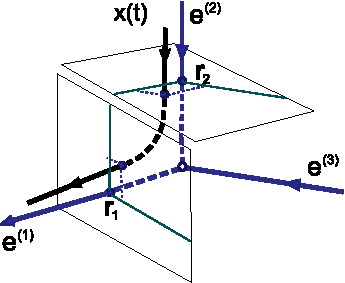
\includegraphics[width=0.45\textwidth]{eqbHypbLin}
 % source in /dasbuch/book/FigSrc/top/A17.*
 \setlength{\unitlength}{0.45\textwidth}
 \begin{picture}(1,0.75806952)%
    \put(0,0){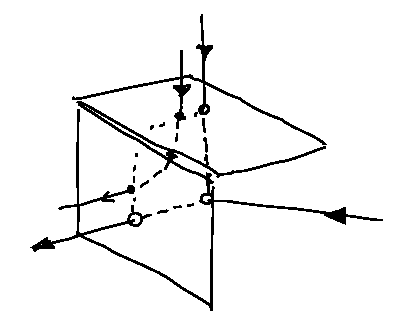
\includegraphics[width=\unitlength]{A17.pdf}}%
    \put(0.36817736,0.66084022){\color[rgb]{0,0,0}\makebox(0,0)[lb]{\smash{$\ssp(t)$}}}%
    \put(0.50066957,0.71553235){\color[rgb]{0,0,0}\makebox(0,0)[lb]{\smash{$\jEigvec[2]$}}}%
    \put(0.90162585,0.24424498){\color[rgb]{0,0,0}\makebox(0,0)[lb]{\smash{$\jEigvec[3]$}}}%
    \put(-0.00199914,0.19101427){\color[rgb]{0,0,0}\makebox(0,0)[lb]{\smash{$\jEigvec[1]$}}}%
    \put(0.32517548,0.15725803){\color[rgb]{0,0,0}\makebox(0,0)[lb]{\smash{$\mathbf{r}_1$}}}%
    \put(0.52100813,0.46373593){\color[rgb]{0,0,0}\makebox(0,0)[lb]{\smash{$\mathbf{r}_2$}}}%
 \end{picture}%
\caption{Linearization of a flow near to an equilibrium:
  the flow is reduced to an analytic map between two
  near Poincar\'e sections, mapping the in-flow into out-flow.
  }\label{f:eqbHypbLin}
\end{figure}
